\documentclass[12pt, a4paper]{article} % Document font size and paper size
\usepackage[utf8]{inputenc}
\usepackage{DejaVuSans}
\usepackage{graphicx}
\usepackage{epstopdf}
\usepackage{multicol}
\usepackage{color}
\usepackage{framed}
\usepackage[usenames,dvipsnames,svgnames,table]{xcolor}
\usepackage{hyperref}
\usepackage{geometry} % Allows the configuration of document margins
\usepackage{color}
\usepackage{listings}
\usepackage[T1]{fontenc}
\usepackage{eurosym}

\usepackage{titlesec}

%\usepackage[protrusion=true,expansion=true]{microtype} % Better typography

\definecolor{orange}{HTML}{FF9900}
\definecolor{shadecolor}{RGB}{150,150,150}
  
\graphicspath{ {./images/} }

\geometry{a4paper, textwidth=6.5in, textheight=8in, marginparsep=6pt, marginparwidth=.6in} % Document margin settings

\lstset{literate=%
    {Ö}{{\"O}}1
    {Ä}{{\"A}}1
    {Ü}{{\"U}}1
    {ß}{{\ss}}2
    {ü}{{\"u}}1
    {ä}{{\"a}}1
    {ö}{{\"o}}1
}

\hypersetup{
 pdfauthor={Schumilin, Tseyzer},
 pdftitle={Seminararbeit}
 pdfsubject={Seminararbeit},
 pdfkeywords={Not set}
}

\hyphenation{
wirt-schaft-liche
wissen-schaft-liche 
Wäh-rend
Un-ter-nehm-en
Fin-anz-ver-wal-tung
Wiss-en-schaft-ler
durch-zu-führ-en
in-ge-nieur-wis-sen-schaft-lich
Ver-öf-fent-lich-un-gen
}

\renewcommand{\figurename}{Abbildung} 
\renewcommand{\tablename}{Tabelle} 
\newcommand{\specialcell}[2][c]{%
  \begin{tabular}[#1]{@{}c@{}}#2\end{tabular}}

\renewcommand*{\familydefault}{\sfdefault}



\titleformat{\section}
{\color{orange}\normalfont\LARGE\bfseries}
{\color{orange}\thesection}{1em}{}
[
\vspace{0.5ex}%
\rule{\textwidth}{2pt}
\vspace{2ex}%
] % after-code

\titleformat{\subsection}
{\color{orange}\normalfont\large\bfseries}
{\color{orange}\thesubsection}{1em}{}

\titleformat{\subsubsection}
{\color{orange}\normalfont\normalsize\bfseries}
{\color{orange}\thesubsubsection}{1em}{}
\begin{document}

%%%%%%%%%%%%%%%%%%%%%%%%%
% TITEL
%%%%%%%%%%%%%%%%%%%%%%%%%
\thispagestyle{empty}

\begin{titlepage}
%%\let\footnotesize\small \let\footnoterule\relax
\begin{center}

\hbox{}
\vskip 1.8cm


\includegraphics[width=0.6\textwidth]{./logo}~

\hbox{}
\vfill
\vskip 1cm
Business Plan\\
von\\[2mm]
\vskip 1cm

{\large\bfseries Artem Schumilin \& Igor Tseyzer\\}
\vskip 4cm
{\bfseries Seminar}\\
Developing Business Models \\
for the Semantic Web (WS 13/14) \\
%Universität Karlsruhe (TH)\\[2ex]
\vskip 2cm

\vskip 1cm
Januar 2014

\end{center}
\vfill
\end{titlepage}

%%%%%%%%%%%%%%%%%%%%%%%%%
% CONTENT
%%%%%%%%%%%%%%%%%%%%%%%%%

\tableofcontents
\newpage

%%%%%%%%%%%%%%%%%%%%%%%%%
% Executive Summary Artem und Igor
%%%%%%%%%%%%%%%%%%%%%%%%%
\section{Executive Summary}

\textsc{\color{orange}{SemLit}} revolutioniert die Literaturrecherche in der überwältigenden Informationsflut unserer Wissensgesellschaft. Mit uns automatisieren Sie Ihre Literaturrecherche und verpassen nie mehr eine interessante Veröffentlichung aus Ihrem Fachgebiet. 
\\
\\
Basierend auf weltweit führender {\color{orange}{Semantischer Technologie}} stellt SemLit eine leistungssarke Web-Plattform für Wissensarbeiter zur Verfügung. Bei uns können Forscher, Studenten und kommerzielle F\&E-Abteilungen ihren persönlichen, virtuellen Literatur-Assistenten trainieren, der für sie maßgeschneiderten Content zur richtigen Zeit und im richtigen Kontext liefert. 
\\
\\
Als erster Anbieter für semantisches Information Retrieval positioniert sich SemLit auf dem Markt für IT- und ingenieurwissenschaftliche Veröffentlichungen und bedient eine {\color{orange}{stark wachsende Zielgruppe}} von Individuen und Institutionen der öffentlichen sowie privaten Forschung. Die technologische Grundlage ist dabei gut skalierbar und soll in Zukunft mit geringem Aufwand auf neue Informationsfelder wie Finanzen, Börsenhandel oder Recht erweitert werden. Eine erfolgreiche {\color{orange}{Monetarisierung}} ergibt sich durch ein System von Abonnements, zielgerichteter Kontext-Werbung und Sponsoring-Verträge mit Firmen und Universitäten. 
\\
\\
Das {\color{orange}{Gründerteam}} von SemLit bringt umfassendes praktisches und theoretisches Know-How auf dem Gebiet Semantischer Technologien mit und ergänzt es durch belegbare  betriebs-wirtschaftliche Kompetenzen. Zusätzlich stehen den Gründern renommierte Partner aus der universitären Forschung zur Seite.
\\
\\
\begin{table}[h!]
  \centering
  \begin{large}
	\begin{itshape}
  \begin{tabular}{c}\hline
  \\
  {\color{orange}SemLit wird die mühsame Praxis der Literatursuche radikal vereinfachen.}\\
  {\color{orange}Lesen Sie im Folgenden, wie diese Revolution vonstatten gehen soll.}\\
  \\\hline
  \end{tabular}
 	\end{itshape}
  \end{large}
\end{table}


\newpage

%%%%%%%%%%%%%%%%%%%%%%%%%
% Geschäftsidee Artem
%%%%%%%%%%%%%%%%%%%%%%%%%
\section{Geschäftsidee}


\subsection{Worum es hier geht}
Eine Studie von International Data Corporation (IDC, eines der führenden Marktforschungsunternehmen in der IT-Industrie) aus dem Jahr 2005\footnote[1]{\textit{White Paper on Hidden Cost of Information Work}, IDC, 2005.} hat gezeigt, dass ein Wissensarbeiter im Durchschnitt rund ein Viertel seiner Arbeitszeit alleine auf die Informationssuche aufwendet. In der wissenschaftlichen Forschung ist dieser Anteil unseren Schätzungen zufolge noch größer. Gesucht wird dabei vor allem nach Information in Form von wissenschaftlichen Publikationen. Weil Publikationen im Idealfall den Stand der Technik abbilden, ist deren Studium ein Grundpfeiler erfolgreicher wissenschaftlicher Praxis. 

\begin{table}[h!]
  \centering
  \begin{large}
	\begin{itshape}
  \begin{tabular}{c}\hline
	\\
  {\color{orange}„Wenn ich weiter geblickt habe, so deshalb,} \\ 
	{\color{orange}weil ich auf den Schultern von Riesen stehe.“} \\
	{\hfill \color{orange}\textit{Isaac Newton, 1676} } \\
	\\\hline
  \end{tabular}
	\end{itshape}
  \end{large}
\end{table}

Neben den obligatorischen Veröffentlichungen in Journals und Konferenzbändern bergen Blogs und Magazine häufig eine nicht minder wichtige Quelle für neue Ideen und Herangehensweisen. An dieser Stelle kommen allerdings vier wichtige Faktoren ins Spiel, die eine erfolgreiche Literaturrecherche erheblich erschweren: 

\begin{description}
  \item[\textbf{\color{orange}{Informationsuniversum wächst:}}] \hfill \\
  Die Zahl möglicher Quellen und potentiell wertvoller Informations-Items wächst rasant: 
In 2008 erschienen allein in den neun\footnote[2]{Nach UNESCO Science Report 2010: GER, FRA, UK, RUS, JPN, KOR, CHN, CAN, USA} großen Wissenschaftsnationen 760.671 Veröffentlichung. Bei der gegenwärtigen jährlichen Wachstumsrate von 3,26\% wird sich diese Zahl in zwanzig Jahren verdoppeln. 
  \item[\textbf{\color{orange}{Information veraltet:}}] \hfill \\
  Neu produziertes Wissen veraltet heute schneller als jemals zuvor. Neue Entwicklungen in einem Forschungsfeld werden schnell entdeckt, aufgegriffen und weiterentwickelt. Wenn man Fortschritt erzielen möchte, ist jede Verzögerung bei der Informationssuche ein schwerwiegender Nachteil. 
  \item[\textbf{\color{orange}{Wissensgebiete werden vernetzt:}}] \hfill \\
  Die Grenzen zwischen den Disziplinen verschwimmen zunehmend. Bahnbrechende Arbeiten über Datenverarbeitung werden manchmal in Biologie-Journals publiziert, weil beispielsweise die Genomforschung ohne Informatik nicht mehr auskommt. Solche potentiell interessanten Informations-Events bleiben natürlich unentdeckt, wenn man die Aufmerksamkeit unmittelbar auf das eigene Feld beschränkt. 
 \item[\textbf{\color{orange}{Verfügbare Such-Tools sind unzulänglich:}}] \hfill \\
	Die Möglichkeiten der Suche in der globalen Informationswolke, bereitgestellt durch Incumbents wie Google und Microsoft, sind weitgehend auf Schlüselworte beschränkt. Dabei ist die Suche nach Bedeutungs-Nuancen und Konzepten das, was eine effektive Literaturrechere ausmacht. 
\end{description} Diese Probleme wird \textsc{\color{orange}{SemLit}} lösen. Mit semantischen Technologien werden wir die Praxis der Literaturarbeit umkrempeln. Im Folgenden beschreiben wir, wie das im Detail geschehen soll. 

\begin{table}[h!]
  \centering
  \begin{large}
	\begin{itshape}
  \begin{tabular}{c}\hline
  \\
  {\color{orange}Ein Wissensarbeiter verbringt durchschnittlich }\\
  {\color{orange}24\% seiner Zeit mit Informationssuche.}\\
  \\\hline
  \end{tabular}
	\end{itshape}
  \end{large}
\end{table}


%=======================================

\subsection{Know-how Träger}
Die Idee und Umsetzung wird von zwei Studenten des Karlsruher Instituts für Technologie (KIT) entwickelt. {\color{orange}Artem Schumilin} studiert Wirtschaftsingenieurwesen (M.Sc) und {\color{orange}Igor Tseyzer} studiert Informationswirtschaft (B.Sc). Wahrend des Studiums am KIT haben beide Gründer die notwendigen Kenntnisse in Web- und Semantic-Web-Technologien gesammelt, was als stabiles Fundament für den Aufbau und weitere Entwicklung der Firma dienen soll. 
\begin{figure}[h!]
\centering

\includegraphics[width=0.6\textwidth]{jsi-aifb-logo}
\end{figure}
\emph{<hier: Liste relevanter Fähigkeiten und Erfahrungen>}
Igor wird im neuen Unternehmen die Marketingstrategie entwickeln und den Vertrieb organisieren, während Artem Verantwortung für die Produktentwicklung und die Finanzen übernehmen wird. 
\\
\\
Neben dem KIT-eigenen Gründernnetzwerk stehen den Gründern renommierte Partner aus der Forschung zur Seite: 
Das Josef-Stefan-Institut (JSI) hat mit Enrycher die weltweit führende \emph{named entity recognition engine} entwickelt und tritt damit als der Tchnologiepartner von SemLit auf. 
Das Institut AIFB des KIT erweist sich erfahrener Mentor in Sachen Ausgründung im Bereich semantischer Technologie und wird das Start-Up mit seinen Kontakten und Rat unterstützen.

%=======================================

\subsection{Innovation}

\textsc{Schritt 0:} wo es beginnt\\
Wir beginnen bei den Informations-Items, die im Internet zur freien Verfügung stehen. Dazu gehören vor allem die Abstracts von wissenschaftlichen Veröffentlichungen aus Journals und Konferenzbänden aber auch Artikel in relevanten Blogs und Online-Magazinen. Die Vielzahl der Quellen wird automatish überwacht, um die Nahezu-Echtzeit-Anforderung erfüllen zu können.\\
{\color{orange}Unsere Kunden können die Auswahl der Quellen auf ihre individuellen Bedürfnisse anpassen. }
\\
\\
\textsc{Schritt 1:} die Semantik hinter dem Text\\
Der Kerngedanke hinter SemLit gründet auf den Möglichkeiten, die durch semantische Repräsentation von Textinformation entehen. Dazu gehört die Erkennung von named entities und ihrer Beziehungen untereinander. Mit JSI's Enrycher steht uns die derzeit weltbeste Technologie bereit, mit deren Hilfe wir die Extraktion semantischer Information aus Textdokumenten realisieren. 
\\
\begin{figure}[h!]
\centering
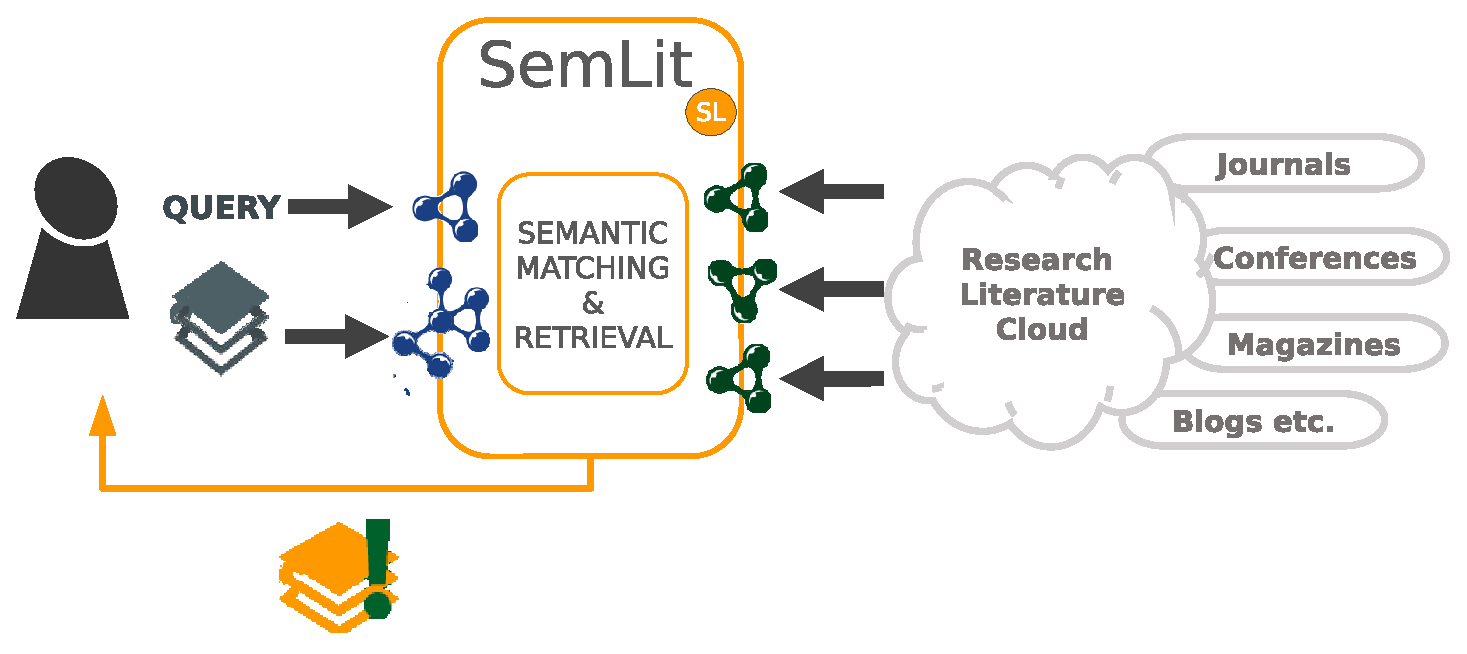
\includegraphics[width=0.9\textwidth]{idea}
\caption{Funktionsschema von SemLit}
\label{fig:idea}
\end{figure}
\\
\textsc{Schritt 2: Informationswunsch äußern}\\
Wie die Textinformation auf der einen Seite, können auf der anderen Seite auch die Suchanfrage der Kunden semantisch repräsentiert werden. Damit kann der Benutzer extrem nuancierte Konzepte ausdrücken. 
Dieses semantische \emph{information retrieval} liefert deutlich bessere Ergebnisse als die gewöhnliche Schlüsselwortsuche alleine. Schlüsselworte sind oft mehrdeutig und liefern damit irrelevante Suchergebnisse, die unnötig Zeit kosten. \\
{\color{orange}Bei SemLit sucht der Benutzer nicht nach einem Wort, sondern nach dem Sinn, der hinter diesem Wort steckt.}
\\
\\
\textsc{Schritt 3: wir gehen weiter als die Anderen}\\
Wir bleiben keineswegs bei den Suchanfragen stehen, sondern gehen noch einen Schritt weiter: Nichts sagt mehr über das Suchinteresse eines Benutzers aus als seine bestehende Dokumentsammlung. Warum also nicht daraus lernen? --- Bei SemLit hat der Kunde die Möglichkeit, ein individuelles System durch Hochladen eigener Dokumente zu trainieren.
\\
\\
{\color{orange}Unter dem Strich entsteht eine Webplattform zur automatischen und individuellen Überwachung der Informationslandschaft. Das System weiß, was der Benutzer will und informiert ihn rechtzeitig, wenn die passende Publikation, ein Blogeintrag oder News-Artikel in Web auftaucht.}

%=======================================

\subsection{Produkt}
SemLit soll in Form einer Web-Applikation und einer App für mobile Geräte an die Kunden ausgeliefert werden. In den nachfolgenden Abbildungen \ref{fig:app} und \ref{fig:website} erklären Entwürde die wichtigsten Komponenten der Funktionalität. 
\\
\begin{figure}[h!]
\centering
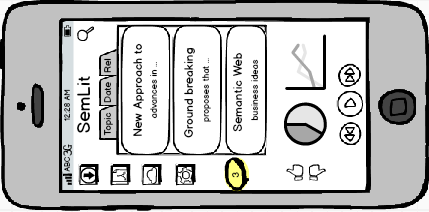
\includegraphics[width=0.5\textwidth]{app}
\caption{SemLit mobile App aggregiert die Funktionalität des Webportals auf kleinem Raum.}
\label{fig:app}
\end{figure}
\\
\\
\\
\begin{figure}[h!]
\centering
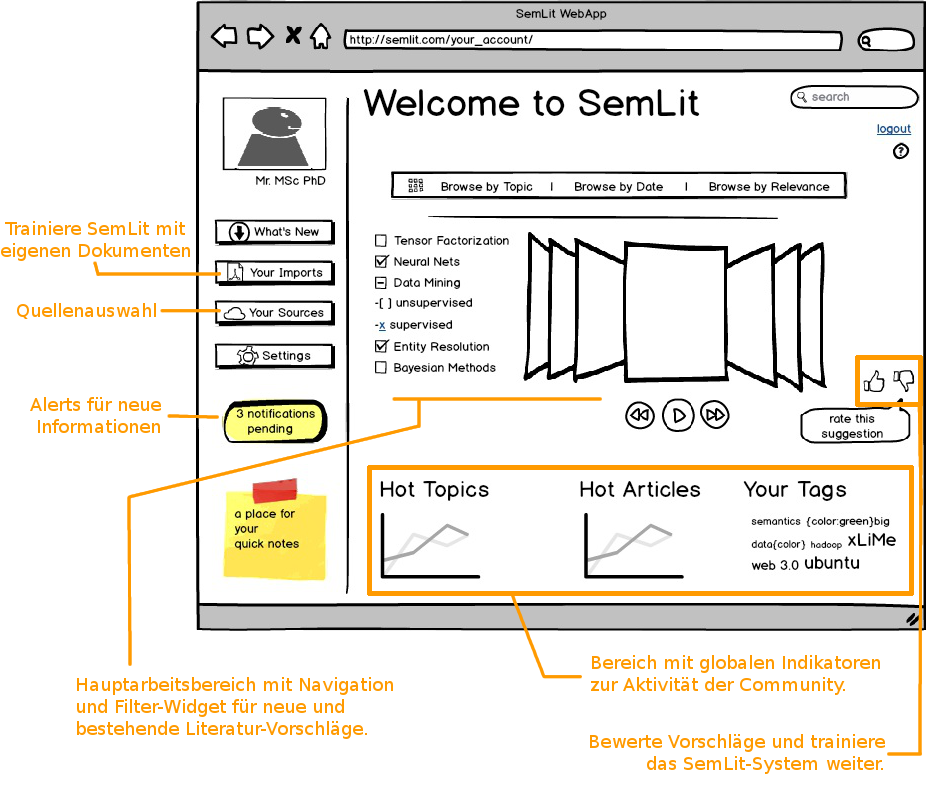
\includegraphics[width=1\textwidth]{website}
\caption{SemLit Webportal mit Erläuterungen zu den wichtigsten Komponenten der Funktionalität.}
\label{fig:website}
\end{figure}

\newpage
%=======================================

\subsection{Customer Value Proposition}
Das Problem mühsamer und zeitraubender Literaturrecherche besteht schon seit es wissenschaftliches Arbeiten gibt. SemLit ist der erste Service auf dem Markt, der dieses Problem durch weitgehende Automatisierung mit semantischen Technologien löst. 
\\
Eine regelbare Vielzahl an Quellen wird durch ein lernfähiges System analysiert und überwacht. Durch SemLit ergeben sich also konkrete Vorteile für den Kunden:
\begin{itemize}
\item Hohe Qualität der Suchergebnisse durch Semantik
\item Neue, potentiell interessante Ergebnisse aus angrenzenden Fachgebieten werden mitgeliefert
\item Informationssuche wird automatisiert
\item Nahezu-realtime Benachrichtigung über neue Veröfentlichungen
\item System passt sich dem Benutzer durch Lerneffekte an und wird mit der Zeit noch besser
\end{itemize}

Die Verbesserung aus diesen Faktoren lässt sich wiederum in Zahlen fassen: Wenn man auf die zuvor erwähnte Studie des IDC (2005) zurückgreift, kann ein Wissensarbeiter demnach mindestens 25\% seiner Zeit einsparen, indem er die Informationssuche mit SemLit weitgehend automatisiert. Für den Arbeitgeber bedeutet das eine geldwerte Ersparnis in Höhe von über 10.000\euro  pro Jahr\footnote[4]{Ausgehend vom bundesweiten monatlichen Durchschnittsgehalt von 3.600\euro  brutto.}. 

%=======================================


\subsection{Unternehmensplanung}

\subsubsection{Rechtliches}
Das Gründerteam wählt die mimi-GmbH als Rechtsform für die Anfangsphase der Unternehmung. Ein Vorteil davon sind die geringeren Kosten der Anmeldung und Anfangsfinanzierung. Im Laufe der nächsten zwei Jahre wird durch periodische Einstellungen ins Eigenkapital die Rechtsform der vollwertigen GmbH erreicht. 
\\
Beide Gründer sind Gesellschafter und nehmen die Verantwortung ebenfalls zu gleichen Teilen als Geschäftsführer wahr.

%=======================================

\subsubsection{Meilensteine}
Wir identifizieren fünf wichtige Events und Prozesse innerhalb der ersten zwei Jahre nach der Gründung. Sie sind auch deshalb bedeuteund, weil sie als Umbruchpunkte im Finanzplan behandelt und abgebildet werden.\\
\begin{description}
  \item[\textbf{1. Offizieller Start}] \hfill \\
In den ersten Wochen sollen vor allem die rechtlichen Einzelheiten geregelt werden. Das wird mit kompetenter Begleitung des Centers für Innovation und Entrepreneurship (CIE) des KIT erfolgen. Das CIE verfügt über Erfahung in diesem Bereich und kann den Kontakt zu bewährten Steuerberatern, Anwäten und weiteren wichtigen Ansprechpartnern empfehlen. In dieser Phase soll die Anmeldung des GmbH-Sitzes, die Registrierung und Eintragung der GmbH ins Handelsregister vorgenommen werden. 
\\
  \item[\textbf{2. Produktionsgrundlage}] \hfill \\
Damit die nachfolgende Produktentwicklung einsetzen kann, müssen die Rechenkapazitäten und Lizenzen erworben werden. Die Rechenkapazitäten werden kostengünstig und flexibel bei {\color{orange}Amazon Web Services} eingekauft. Das Gründerteam verfügt bereits über praktische Erfahrung im Umgang mit dem IaaS-Angebot von Amazon und kann diese Technologien gut einschätzen. 
\\
Der zweite wichtige Teil dieser Phase umfasst den Erwerb einer Lizenz für \emph{Enrycher}\footnote[3]{Test-Version zu finden als Web-Service unter http://enrycher.ijs.si}, das semantische Textanalyse-Werkzeug des AI-Laboratoriums unseres Technologiepartners JSI. Erster Kontakt zu den Verantwortlichen auf der Seite von JSI konnte über unseren Mentor, das AIFB-Institut, bereits erfolgreich hergestellt werden.
\\
  \item[\textbf{3.1. Produktentwicklung}] \hfill \\
Die ersten 4 Monate nach Kick-Off sind für die Produktentwicklung veranschlagt. Dabei soll die Aufgabe der Frontend-Entwicklung (Infrastruktur und Interface der mobilen Anwendung und der Web-App) an einen geeigneten Dienstleister ausgelagert werden. So kann sich das Gründerteam der Entwicklung der SemLit-Kernkompetenz rund um die Beschaffung, Verwaltung und Analyse der Daten widmen. Damit wird die Time-to-Market signifikant verringert.  
\\
  \item[\textbf{3.2. Marketing \& Kundenaquise}] \hfill \\
Während der letzten Entwicklungsphase werden bereits die ersten Marketing-Kampagnen gestartet. Zunächst sollen verstärkt Privatkunden auf Konferen und durch Social-Media-Marketing geworben werden. 
\\
Basierend auf dem Feedback der beta-Kunden werden wir das System verbessern und im Anschluss darauf offensiv um Firmenkunden werben. Zu diesem Zeitpunkt wird ein Kundensupport-Mitarbeiter zum Team stoßen, um eine bessere Betreuung bei Wünschen und Problemen zu gewährleisten.
\\
  \item[\textbf{4. Wachstum}] \hfill \\
Damit das Team adequat die Anregungen und Verbesserungsvorschläge der Benutzer einarbeiten kann, sollte im zweiten Quartal des zweiten Jahres eine feste Developer-Stelle besetzt werden. Das Angebot muss ständig weiterentwickelt und an Kundenwünsche angepasst werden.
\\
  \item[\textbf{5. Break-Even}] \hfill \\
Im Fall von SemLit sind die Kosten der Anfangsphase relativ gut prognostizierbar. Außerdem sind die bedeutsamen Kostenarten (Personal-, Betriebs-, Lizenzkosten) wenig volatil. Damit wird im neutralen Umsatz-Szenario der Break-Even-Punkt schätzungsweise in Q2 des zweiten Geschäftsjahres erreicht. Weitere Details werden im Abschnitt Finanzplanung diskutiert. 
\end{description}








\newpage

%%%%%%%%%%%%%%%%%%%%%%%%%
% Analyse des Marktes Igor
%%%%%%%%%%%%%%%%%%%%%%%%%
\section{Analyse des Marktes}


\subsection{Zielgruppe und potenzielle Kunden}
SemLit richtet sich auf alle, die in der wissenschaftliche Bereich tätig sind. Semlit ist eine Dienstleistung, die Wissenschaftler in unterschiedliche Bereichen der Forschung und Entwicklung unterstützen wird. Die Konsumenten könnten in drei Gruppen gegliedert werden:
\begin{itemize}
\item Private Personen (Studenten und Wissenschaftler)

\item Wissenschaftliche Einrichtungen (Universitäten, Forschungszentren)

\item Unternehmen (Forschungs- und Entwicklungsabteilungen)
\end{itemize}

\subsection{Marktsituation}
Die Marktanalyse wird auf Basis von UNESCO Science Report 2010 durchgeführt. Dieser Bericht stellt wichtige Daten über die Große, potenzielle Entwicklungsrichtungen und Wachstum der Wissenschaft zusammen.\\
Die Endnutzer der SemLit sind Wissenschaftler, deswegen  die potenzielle Entwicklungsrichtungen des Marktes aus Daten über Anzahl der Wissenschaftler in der Welt abgeleitet werden können. In der Bericht von UNESCO kann man die Daten für 2002 und 2007 Jahre finden und Wachstum schätzen.\\

\begin{table}[h!]
  \centering
  \begin{large}
  \begin{tabular}{c}\hline
  \\
  {\color{orange}Anzahl der Wissenschaftler in der Welt}\\
  {\color{orange}hat sich in 5 Jahren von 5 810 700}\\
  {\color{orange}auf 7 209 700 Wissenschaftler erhöht}\\ 
  \\\hline
  \end{tabular}
  \end{large}
\end{table}

Wie kann man aus Abbildung \ref{fig:fig1} sehen, der gesamte Anzahl der Wissenschaftler in der Welt hat sich von 5 810 700 auf 7 209 700 Wissenschaftler erhöht, was entspicht ein Wachstum um ca. 24\% in 5 Jahren. Die größte Anteil sind die Wissenschaftler aus entwickelten Länder, aber Entwicklungsländer zeigen größere Wachstumspotenzial in Höhe von ca. 55,5 \% in 5 Jahre, gegen ca. 10,6\% Wachstum für entwickelten Länder.\\
\begin{figure}[h!]
\centering
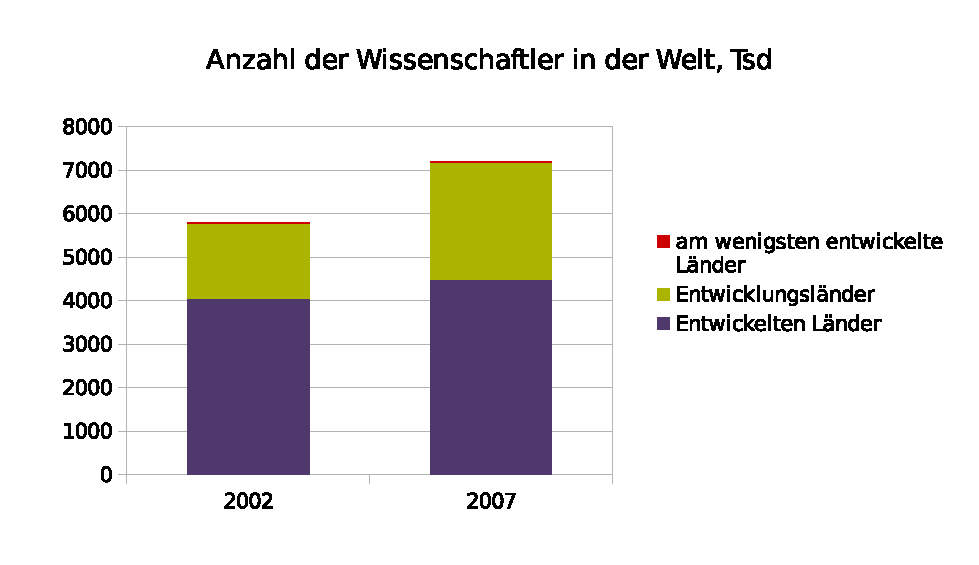
\includegraphics[width=0.8\textwidth]{fig1}
\caption{Anzahl der Wissenschaftler in der Welt, UNESCO 2010}
\label{fig:fig1}
\end{figure}
Andere Daten, die oben genannte Tendenz bestätigen, sind die Anzahl der Publikationen in der Welt. In 6 Jahre hat sich die Anzahl der Publikationen von 733305 auf 986099 erhöht, was ca. 34,5\% der Erhöhung entspricht. Die größte Anzahl gehört zur entwickelten Länder, aber Entwicklungsländer zeigen signifikante 105,9\% Wachstum (Abbildung \ref{fig:fig2})\\
\begin{figure}[h!]
\centering
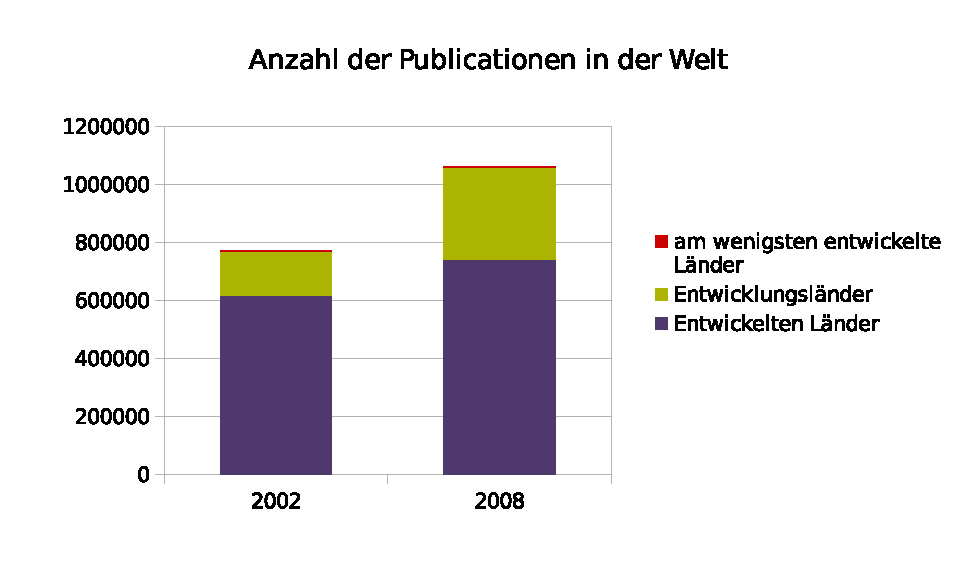
\includegraphics[width=0.8\textwidth]{fig2}
\caption{Anzahl der Publikationen in der Welt, UNESCO 2010}
\label{fig:fig2}
\end{figure}
Auf Grund dieser Daten, kann man feststellen, dass  wichtige Märkte sich in entwickelte Länder befinden. Die Entwicklungsländer zeigen aber riesige Wachstumspotenzial und sollte auch berücksichtigen werden. 
Als Zusammenfassung kann man sagen, dass die Markt der Potenzielle Kunden in letzte Jahren eine gute Wachstum gezeigt hat und eine gute Aufsicht auf weitere Entwicklung besitzt.

\subsection{Auswahl der regionale Märkte}
Auswahl von regionale Märkte ist wichtige Teil der Marketingstrategie. Konzentration auf nur begrenzte Liste der regionale Märkte lasst die  regionale Eigenschaften berücksichtigen und möglichst beste Dienstleistung anzubieten. Enge Zusammenarbeit auf regionale Markt und Partnerprogrammen sollten Erfolg der Absatz unterstützen und neue Richtungen in Entwicklung darstellen.\\
Um richtige regionale Märkte auszuwählen, wird es nur die Länder ausgewählt, die maximale Anzahl der Wissenschaftler haben, da die Wissenschaftler die Endnutzer der SemLit sind. \\
Das Auswahl der Länder erfolgt mit Hilfe der Angaben von UNESCO 2010 über die Anzahl der Wissenschaftler in jedes Land. Es wird nur die Länder ausgewählt, die zusammen ca. 70\% von der gesamte Anzahl alle Wissenschaftler in der Welt bauen. Die Zusammenfassung der Entwicklung der Anzahl der Wissenschaftler ist in der Tabelle \ref{tab:ABC} dargestellt.\\
\begin{table}[h!]
  \centering
  \begin{large}
  \begin{tabular}{c}\hline
  \\
  {\color{orange}acht ausgewählte Länder bauen}\\
  {\color{orange}ca. 70\% von alle Wissenschaftler in der Welt}\\
  \\\hline
  \end{tabular}
  \end{large}
\end{table}
Wie kann man aus Tabelle \ref{tab:ABC} sehen, acht ausgewählte Länder bauen ca. 70\% von alle Wissenschaftler in der Welt. Viele von denen zeigen auch signifikante Erhöhung um mehr als 50\% in 5 Jahre. Dieser Länder sind China und Südkorea.


\begin{table}[h!]
  \centering
  \begin{footnotesize}
  \begin{tabular}{|l|r|r|r|r|r|}\hline
  \textbf{Land} & \multicolumn{4}{ c| }{\textbf{Anzahl der Wissenschaftler, Tsd.}} & \textbf{Wachstum}\\
  & 2002 & \% gesamt & 2007 & \% gesamt & \\ \hline
Welt & 5810.7 & 100.00\% & 7209.7 & 100.00\% & 24.08\% \\ \hline
Vereinigte Staaten & 1342.5 & 23.10\% & 1425.6 & 19.77\% & 6.19\% \\
China & 810.5 & 13.95\% & 1423.4 & 19.74\% & 75.62\% \\
Japan & 646.5 & 11.13\% & 710 & 9.85\% & 9.82\% \\
Russische Föderation & 491.9 & 8.47\% & 469.1 & 6.51\% & -4.64\% \\
Deutschland & 265.8 & 4.57\% & 290.9 & 4.03\% & 9.44\% \\
Vereinigtes Königreich & 198.2 & 3.41\% & 254.6 & 3.53\% & 28.46\% \\
Südkorea & 141.9 & 2.44\% & 221.9 & 3.08\% & 56.38\% \\
Frankreich & 186.4 & 3.21\% & 215.8 & 2.99\% & 15.77\% \\
Kanada & 116 & 2.00\% & 139 & 1.93\% & 19.83 \% \\ \hline
Alle ausgewählte Länder & 4199.7 & 72.28\% & 5150.3 & 71.44\% & 22.63\% \\ \hline
  \end{tabular}
  \end{footnotesize}
  \caption{Länder mit größte Anteil der Wissenschaftler, basiert auf Daten von UNESCO 2010}
  \label{tab:ABC}
\end{table}


Für alle ausgewählte Länder wird andere wichtige Parameter geschätzt, Bruttoinlandsausgaben für Forschung und Entwicklung (GERD) pro ein Wissenschaftler. Dieser Parameter könnte zeigen, wie viel Geld in der Forschung und Entwicklung investiert wird. Je mehr dieser Zahl ist, desto mehr ist die Wahrscheinlichkeit, dass Wissenschaftler das Geld nicht nur für reine Forschung, sonder auch für Dienstleistung, die dieser Forschung erleichtern könnten, zahlen werden. In Tabelle \ref{tab:ABC2} sind die Angaben zum Entwicklung der Bruttoinlandsausgaben für Forschung und Entwicklung pro ein Wissenschaftler präsentiert. Wie kann man aus Tabelle \ref{tab:ABC2} sehen, entwickelte Länder investieren sehr viel Geld in Forschung und Entwicklung, was als gute Möglichkeit für Absatz sprechen kann. 
\begin{table}[h!]
  \centering
  \begin{footnotesize}
  \begin{tabular}{|l|p{3cm}|p{3cm}|r|}\hline
  \textbf{Land} & \multicolumn{2}{ r| }{\textbf{GERD pro Wissenschaftler, \$ Tsd.}} & \textbf{Wachstum} \\
  & 2002 & 2007 & \\ \hline
Deutschland & 213.1& 248.4 & 16.56\% \\
Vereinigte Staaten & 206.4 & 243.9 & 18.17\% \\
Japan & 167.3 & 208.4 & 24.57\% \\
Frankreich & 204.7 & 196.1 & -4.20\% \\
Südkorea & 158.6 & 186.3 & 17.47\% \\
Kanada & 165 & 170.7 & 3.45\% \\
Vereinigtes Königreich & 154.6 & 152.2 & -1.55\% \\
China & 48.4 & 72 & 48.76\% \\
Russische Föderation & 32.4 & 50.1 & 54.63\% \\ \hline
  \end{tabular}
  \end{footnotesize}
  \caption{Bruttoinlandsausgaben für Forschung und Entwicklung (GERD) pro ein Wissenschaftler, basiert auf Daten von UNESCO 2010}
  \label{tab:ABC2}
\end{table} 



\subsection{Schätzung der Marktvolumen}
Schätzung der Marktvolumen ist für Bereich Wissenschaft schwierig, da genauer Daten über die Anzahl und Budget nicht die Realität abbilden können. Deswegen werden dieser Daten grob aus vorhandene Daten abgeleitet. Zuerst wird die gesamt Anzahl der Wissenschaftler und Bruttoinlandsausgaben für Forschung und Entwicklung in ausgewählte regionale Märkte berechnet. Dann Anzahl von alle Publikationen und Anzahl von Publikationen in Bereich von Ingenieurwesen und Technologie, die in dieser Länder publiziert worden. 
\begin{table}[h!]
  \centering
  \begin{large}
  \begin{tabular}{c}\hline
  \\
  {\color{orange}Verhältnis von der Anzahl der Wissenschaftler}\\
  {\color{orange}zur Anzahl der alle Publikationen ist ca. 7}\\
  \\\hline
  \end{tabular}
  \end{large}
\end{table}
Aus resultierte Daten von Anzahl der Publikationen, könnte ein Verhältnis-Koeffizient berechnet werden, die grobe Schätzung über die Anteil von Ingenieurwesen und Technologie in gesamte Wissenschaftliche Tätigkeit geben kann. Andere Koeffizienten, die wichtig sein könnten, sind Verhältnis von Anzahl der Wissenschaftler / Anzahl der alle Publikationen und Verhältnis von Bruttoinlandsausgaben für Forschung und Entwicklung / Anzahl der alle Publikationen. Dieser Koeffizienten zeigen, dass durchschnittlich 7 Wissenschaftler auf eine Publikation arbeiten und durchschnittliche Bruttoinlandsausgaben für eine Publikation ca. 1137,8 Tsd. von PPP\$ ist.
\begin{table}[h!]
  \centering
  \begin{footnotesize}
  \begin{tabular}{|l|l|}\hline
   \textbf{Parameter} &  \textbf{Wert} \\ \hline
  Anzahl der Wissenschaftler & 5150300 \\ \hline
  Bruttoinlandsausgaben für Forschung und Entwicklung & 865,5 Mrd. PPP\$ \\ \hline
  Anzahl der alle Publikationen & 760671 \\ \hline
  Anzahl der Publikationen in Ingenieurwesen & 101351
 \\
  und Technologie& \\ \hline
  Verhältnis (Publikationen in Ing.\& Tech. / alle Publikationen) & 13,3\% \\ \hline
  Verhältnis (Anzahl der Wissenschaftler / Anzahl der & ca. 7 \\
  alle Publikationen ) & \\ \hline
  Verhältnis (Bruttoinlandsausgaben für Forschung & 1137,8 Tsd. PPP\$\\
  und Entwicklung / Anzahl der alle Publikationen) & \\ \hline
  \end{tabular}
  \end{footnotesize}
  \caption{Angaben zur Märkte, basiert auf Daten von UNESCO 2010}
  \label{tab:ABC3}
\end{table}
 

\subsection{Wettbewerber}
Die wesentliche Wettbewerber, die in der Feld der Akademische Suche sind Suchmaschinen. Normalweise, Suchmaschinen bieten keine Zugang zum Volltext, sondern zur Abstrakt und Referenzen. Wichtige Suchmaschine sind in Tabelle \ref{tab:wettSuch} zusammengefasst.
\begin{table}[h!]
  \centering
  \begin{footnotesize}
  \begin{tabular}{|l|l|l|l|}\hline
   \textbf{Name} &  \textbf{Suchverfahren} &  \textbf{Suchbereiche} &   \textbf{Zugang} \\ \hline
BASE - Bielefeld Academic  & Fast Search \& & Interdisziplinär & Kostenfrei \\
Search Engine & Transfer  & & \\ \hline
 Google Scholar & Eigene & Interdisziplinär & Kostenfrei\\\hline
 Microsoft Academic & Vertikale & Informatik & Kostenfrei \\
 Search & Suchmaschine & & \\ \hline
 CiteSeer & Eigene & Informatik & Kostenfrei \\ \hline
  \end{tabular}
    \end{footnotesize}
  \caption{Wichtige Suchmaschine}
  \label{tab:wettSuch}
\end{table} 
 
Zur zweite Gruppe gehören Datenbanken. Sie stellen nicht nur Suche in Abstrakt und Referenzen, sondern auch Zugang zur Volltexte. Normalweise, Suche und Zugang zum Abstrakt sind kostenfrei. Um Zugang zum Volltext zu bekommen, soll man eine Abonnement kaufen. Wichtige Datenbanken sind in der Tabelle \ref{tab:wettDaten} gelistet. 
\begin{table}[h!]
  \centering
    \begin{footnotesize}
  \begin{tabular}{|l|l|l|l|}\hline
  \textbf{Name} &  \textbf{Suchbereiche} &  \textbf{Zugang} &  \textbf{Anbieter} \\ \hline
 SpringerLink & Interdisziplinar & Abonnement & Springer\\ \hline
 Academic Search & Interdisziplinar & Abonnement & EBSCO Publishing\\ \hline
 IEEE Xplore & Informatik \& & Abonnement & IEEE\\ 
 & Elektrotechnik & & \\ \hline
 Scopus & Interdisziplinar & Abonnement & Elsevier\\ \hline
 Web of Science & Interdisziplinar & Abonnement & Thomson ISI \\ \hline
  \end{tabular} 
    \end{footnotesize}
  \caption{Wichtige Datenbanken}
  \label{tab:wettDaten}
\end{table} 


\subsection{Alleinstellungsmerkmal und Kundennutzen}
Der wesentliche Unterschied zwischen schon existierende Angebote auf Markt und SemLit ist semantische Suche, Verwaltung von Publikationen, Self-Learning Algorithmus, um neue relevante Publikationen zu finden. Auf eine Seite SemLit stellt ein Dienstleistung wie Suchmaschinen auf andere Seite gibt es eine Möglichkeit auf bevorzugte Datenbanken zuzugreifen.\\
SemLit ist sehr flexibel bei Kundennutzung. Wenn die Kunden schon existierende Abonnement für eine der Datenbanken haben, SemLit als eine erweiterte Suchmaschine genutzt werden kann. D.h. Kunden können eine glatte Übergang von vorhandene Lösung zur SemLit durch führen oder SemLit als Erweiterung nutzen. 



\newpage

%%%%%%%%%%%%%%%%%%%%%%%%%
% Marketingstrategien Igor
%%%%%%%%%%%%%%%%%%%%%%%%%
\section{Marketingstrategien}



\subsection{Dienstleistungsformen}

Die Dienstleistung stellt Zugangsformen für Kunden dar:
\begin{itemize}
\item Webauftritt
\item App für Mobile Geräte
\end{itemize}

Die Dienstleistung wird wird vor allem als Webauftritt dargestellt. App für Mobile Geräte ist für Unterstützung der Webauftritt und Erweiterung der Nutzbarkeit und Nutzungserfahrung genutzt.\\

Die Dienstleitung stellt folgende Funktionen zur Verfügung:
\begin{itemize}
\item Sematische Suche der Publikationen
\item Suche in verwandte Felder. 
\item Verwaltung und Auswahl der wissenschaftlicher Suchquellen
\item Gestaltung von eigene Publikationslisten und Share-Funktion.
\item Gestaltung von Literaturverzeichnis für eigene Publikationen und Export-Funktionen in {\LaTeX} und andere Formaten. 
\item Verwaltung genutzter Publikationen
\item Self-Learning Algorithmus zur Verbesserung Suchergebnisse, basiert auf vorher gesuchte Publicationen.
\end{itemize}

Dieser Funktionen sind Anfangsfunktionen und werden durch Kunden-Feedback aktualisiert. 

\subsection{Nutzungsverfahren der Dienstleistung}
Die Dienstleistung für Endnutzer wird auf folgende Bedingungen angeboten:
\begin{itemize}
\item Funktion der Sematische Suche wird auf Webauftritt kostenlos und ohne Anmeldung angeboten
\item Zugang zur andere Funktionen der Dienstleistung erfolgt nur nach der Anmeldung und entsprechend der ausgewählte Nutzungsform. 
\end{itemize}
Dieser Gliederung dient für Kundengewinnung und stellt eine Möglichkeit die Dienstleistung unverbindlich zur nutzen. Die genaue Nutzungsformen werden in der Abschnitt Monetarisierung dargestellt. 

\subsection{Monetarisierung}

Die Monetarisierung wird von zwei Perspektiven Betrachten - direkt und indirekt. Bei direkte Monetarisierung, Geldeinfluss kommt gerade von Kunden. Die Kunden können die Dienstleistung in der Form von Abonnement nutzen. Kunden zahlen feste Preis per Monat für Dienstleistungsnutzung, die in zwei Varianten gegliedert - Basic und Extended. Basic stellt eine Möglichkeit kostengünstig Funktionen "Suche in verwandte Felder" und "Verwaltung und Auswahl der wissenschaftlicher Suchquellen" nutzen. Bei Extended, kann man alle existierende Funktionen unbegrenzt nutzen.\\

Bei indirekte Ansicht wird das Geldeinfluss aus Quellen, die nicht bei Endnutzer sind. Dieser Quellen sind
\begin{itemize}
\item \textbf{Sponsorships}. Geldeinfluss von Unternehmen oder Einrichtungen, die Bekanntheit zu erhöhen oder naher Kommunikation mit bestimmte Kundengruppe gestalten wollen.
\item \textbf{Werbung}. Kontext-basierte Werbung auf Webauftritt.
\end{itemize}

Zusammen direkte und indirekte Monetarisierung stellen eine Möglichkeit eine glatte Geldeinfluss zu gestalten und am schwierige Anfangsphase Finanziell gesichert sein.

 
\subsection{Vertriebskanake und Kommunikation}

Für eine erfolgreiche Markteintritt und Absatz braucht man eine gute Vorbereitung der Vertriebskanake und Kommunikation mit Kunden festzustellen und entsprechend nutzen. Um die Dienstleistung für potenzielle Kunden bekannt zu machen und eine Möglichkeit zu gestalten die Dienstleistung zu nutzen, werden folgende Maßnahmen durchgeführt: 
\begin{itemize}
\item Teilnahme an Konferenzen. SimLit wird auf die große Konferenzen präsentiert, wo jede von potenzielle Kundengruppe die Dienstleistung kostenlos probieren kann.
\item Direkt Verkauf. Ein direkte Besprechung mit Wissenschaftliche Einrichtungen und Unternehmen. Dieser Verfahren sorgt dafür jede einzelne potenzielle Kundengruppe ein gute Ansprechpartner zu sein und Bedürfnisse der Kunden zu berücksichtigen.
\item Partner Programmen. Speziale Angebote für wissenschaftliche Einrichtungen (Rabatte oder kostenlose Zugang) für unsere Partnern in Wissenschaft.
\end{itemize}

\subsection{Markteintrittplan}

Markteintritt kann in vier Phasen gegliedert werden. Alle Phasen sollen Erfolg der Dienstleistung auf den Markt sichern und unterstützen: 
\begin{enumerate} 
\item Vorbereitung
\item Eintritt 
\item Kontrolle 
\item Anpassung 
\end{enumerate}

Wahrend der \textbf{Vorbereitung Phase} wird die Infrastruktur gebaut. Der Markteintritt soll mit schon funktionierte Dienstleistung erfolgen. Zu dieser Phase zahlt noch die Marketingvorbereitungsmaßnahmen. Dieser Phase befasst:
\begin{itemize}
\item Gestaltung der Suchmaschine
\item Anmeldung der Domain für Webauftritt
\item Gestaltung der Markenrichtlinien (Logo, Farben etc.)
\item Werbematerialvorbereitung
\item Gestaltung der Webauftritt und Mobile App
\item Testen der alle Funktionen 
\item Gestaltung der Infrastruktur (Büro, Miete der Rechnerkapazitäten oder Einkauf, Unternehmensrundung, Buchhaltung, Juristische Beratung etc.)
\end{itemize}

Nach der Vorbereitung wird \textbf{Markteintritt} durchgeführt. Dieser Phase ist schwierig und verlangt viel Konzentration und Aufwand. Es wird ausgeführt:
\begin{itemize}
\item Veröffentlichung der Webauftritt 
\item Start der Kommunikationspolitikmaßnahmen und Search Engine Optimization (SEO)
\end{itemize}

Mit Hilfe der \textbf{Kontrolle} kann man alle Parameter, die für Funktionieren der Dienstleistung wichtig sind, kontrollieren und entsprechende Maßnahmen durchzuführen. Man soll die Parameter so zu wählen, dass sie die Wirklichkeit spiegeln. Eine von Parameter könnte sein:
\begin{itemize}
\item Besucheranzahl von Webauftritt 
\item Anzahl der neue Anmeldungen 
\item Anzahl der Suchanfragen
\item Statistik an genutzte Datenquellen
\item Variablenkosten 
\end{itemize}

Zusammen mit der ständige Kontrolle sollte die \textbf{Anpassung} gemacht werden. Alle Maßnahmen soll gut angepasst werden, um maximale Erfolg und Verbesserung der Dienstleistung zu verfolgen.


\newpage

%%%%%%%%%%%%%%%%%%%%%%%%%
% Unternehmensplanung Igor
%%%%%%%%%%%%%%%%%%%%%%%%%
%
\section{Unternehmensplanung}
- geplante Rechtsform und Organisation bzw. Organigramm für das zu gründende Unternehmen

Der erste Mitarbeiter in Ihrem Unternehmen sind zunächst Sie selbst: Beschreiben Sie daher, welche beruflichen Erfahrungen Sie in der Branche gesammelt haben und wie Ihre bisherigen Erfolge aussahen. Haben Sie vielleicht eine Weiterbildung gemacht oder sich auf anderem Wege wertvolles Wissen angeeignet? Wie sieht Ihre Personalplanung für die nächsten drei bis fünf Jahre aus: Wollen Sie überhaupt Mitarbeiter einstellen und wenn ja, wie viele? Wollen Sie vielleicht mit freien Mitarbeitern oder Aushilfen zusammenarbeiten? So wie Sie Ihre eigenen Kenntnisse aufgelistet haben, sollten Sie auch die Qualifikationen Ihrer möglichen Partner und der schon feststehenden Mitarbeiter beschreiben.


%\newpage

%%%%%%%%%%%%%%%%%%%%%%%%%
% Chancen und Risiken Artem
%%%%%%%%%%%%%%%%%%%%%%%%%
\section{Chancen und Risiken}
In diesem Abschnitt diskutieren wir interne Faktoren und externe Umweltbedingungen, die sich positiv auf das Start-Up auswirken, beschreiben aber auch mögliche Risikofaktoren und zeigen, wie \textsc{SemLit} sie bewältigen kann.
\subsection{Stärken}
\textbf{Technologie}\\
Unsere größte Stärke liegt zweifelsohne in der innovativen semantischen Tehcnologie. Dabei konnte sie sich schon in zahlreichen anwendungsorientierten Forschungsprojekten bewähren und hat auch gute Ergebnisse geliefert.
\\
\\
\textbf{Skalierbarkeit und Wachstum}\\
Die angewandte Technologie bringt wiederum den Vorteil mit sich, dass sie sehr gut skaliert und ohne großen Aufwand auf neue Wissens-Domänen angewandt werden kann. Damit hat SemLit das Potential, sich schnell und kostengünstig neuen Kundengruppen zuwenden zu können. So wäre es beispielsweise in naher Zukunft möglich, den Informationsmarkt für Rechts- und Finanzliteratur in den Fokus zu nehmen. Sowohl im einen, als auch im anderen Sektor kann man präzise eine Menge an hoch-qualitativen Online-Quellen für relevante Veröffentlichungen indetifizieren und dazuschalten. Im Ergebnis wäre eine Kundengruppe mit besonders hoher Zahlungsbereitschaft gewonnen.
\\
\\
\textbf{Standort}\\
Bei der gegenwärtigen Lage in Sachen Datenschutz und -sicherheit ist ein Unternehmenssitz in Deutschland von großem Vorteil. Die hohen Standards hierzulande bilden ein überzeugendes Argument, besonders für Kunden aus dem angelsächsischen Raum, und insbesondere angesichts neuester Datenschutzskandale.

\subsection{Schwächen}
\textbf{Recruiting als Start-Up}\\
Als Start-Up ist es nicht einfach, die besten Mitarbeiter anzuwerben. Während die finanzielle Situation keine hohen Gehälter zulässt, stellt die Geschäftslage hohe Arbeitsbelastungen in Aussicht. Diesem Problem wollen wir mit einer wenig rigiden Arbeitszeitplanung und Aussicht auf Erfolgsbeteiligung entgegenwirken. 
\\
\\
\textbf{Kommerzielle Nutzung von Abstracts}\\
Eine weitere Frage erwächst aus der kommerziellen Nutzung von Abstract-Texten. Die Verlage veröffentlichen diese im Normalfall zur unentgeltlichen Nutzung. Ob bei massivem Crawling von Abstracts mit einer Rechtsklage zu rechnen ist, muss beim Rechtsexperten endgültig geklärt werden. \\
Eigentlich ist SemLit aus unserer Sicht letztendlich sogar vorteilhaft für die Verlage, weil es zu weitreichender und einfacher Verbreitung ihrer Publikationen führt.

\subsection{Chancen}
\textbf{Positive Marktstimmung}\\
Der Markt ist bereit für semantische Technologien: Der Gartner-Bericht 2013\footnote[5]{Quelle: http://www.gartner.com/newsroom/id/2359715} erkennt in semantischen Technologien den Schlüssel zur Bewältigung kommender Herausforderungen in der Informationsverarbeitung. Nach unserer Einschätzung gehen damit positive Kunden-Erwartungen, eine geringere Hemmschwelle und auch höhere Zahlungsbereitschaft einher.
\\
\\
\textbf{Exit durch Übernahme}\\
Als stark spezialisiertes Unternehmen in einem hochinnovativen Technologiesegment ist SemLit ein guter Kandidat für die Übernahme durch einen der großen Spieler. Außerdem werden die Vorzeichen einer Übernahme durch die kommende Erholung der Weltkonjunktur begünstigt. Für SemLit ist das die bevorzugte Exit-Strategie.

\subsection{Risiken}
\textbf{Konkurrenz}\\
Der beste Kandidat für einen direkten Konkurrenten wäre Google. Neben massiver technologischer und personeller Kompetenz verfügt Google mit dem Dienst Scholar bereits über die nötige Datengrundlage.\\
Bis jetzt deutet allerdings nichts darauf hin, dass Google Scholar zu einem vergleichbar umfassenden und spezialisierten Angebot ausgebaut werden soll. 
\\
\\
\textbf{Micropayment-Gebühren}\\
Um die Reichweite im Markt zu erhöhen, wird SemLit auf einen Micropayment-Dienstleiter wie PayPal angewiesen sein. Bei jeder Transaktion würdem deshalb entsprechende Gebühren anfallen. Außerdem könnte sich mit der Zeit ihre Höhe ändern.\\
Derzeit verlangt PayPal jedoch einen vertretbaren Aufschlag: Für Zahlungen innerhalb Deutschlands entstehen ca. 2,5\% und international etwa 3-5\% an Umsatzgebühren. Damit ist die starke erhöhte Reichweite bei diesem Stand relativ billig erkauft.

\newpage

%%%%%%%%%%%%%%%%%%%%%%%%%
% Finanzplanung Artem
%%%%%%%%%%%%%%%%%%%%%%%%%

\section{Finanzplanung}
Hier erläutern wir die Hauptkostenarten sowie Einnahmequellen und entsprechende Annahmen, mit deren Hilfe wir zu einer realistischen Einschätzung der Cashflows der ersten zwei Jahre gelangen.
\subsection{Umsatz}
Als Umsatz werden für die Schätzung lediglich die Einnahmen aus den Abonnements betrachtet. Zusätzlich sollten an dieser Stelle auch Werbeeinnahmen addiert werden, die wir jedoch mangels genauer Prognosen weglassen. Es handelt sich hier also um eine konservative Schätzung.\\
Neben den kalkulierten Preisen für private Accounts (1\euro{} basic, 3\euro{} extended) und Firmenkunden (150\euro{} basic, 450\euro{} extended) nehmen wir außerdem je Kundengruppe einen Split von 30-70 für den Kauf der extended- bzw. der basic-Version an. Der Marktanteil wird konservativ mit 1\% angesetzt, was einer realistischen Schätzung für ein Spezial-Start-Up in den ersten 24 Monaten entspricht.
\subsection{Hauptkostenarten}
Im ersten Monat fallen Lizenzkosten in Höhe von 35.000\euro{} an. Dazu kommen relativ geringfügige Fixkosten der GmbH-Anmeldung. In den darauf folgenden 4 Monaten spielen die Kosten des externen Development-Dienstleisters eine wichtige Rolle. \\
Den bei weitem größten laufenden Posten bilden die Personalkosten, gefolgt von den variablen Kosten der IT-Infrastruktur bei Amazon Web Services. 

\subsection{Szenario-Analyse}
Ausgehend von dem Normalfall werden das beste und schlechteste Szenario durch Variation der Umsatzerlöse simuliert. Die Kosten nehmen wir dabei jeweils als konstant an. Von der Besteuerung wird an dieser Stelle abgesehen und stattdessen nur der EBIT betrachtet. Im Überblick zeigt Abbildung \ref{fig:financials1} den Verlauf der Kosten, Umsatzerlöse und des Gewinns vor Steuern und Abschreibungen (EBIT) im neutralen Umsatzszenario. \\
Für jedes Szenario ist die Lage des Break-Even-Punktes von besonderem Interesse (Tabelle \ref{tab:break-even}):
\\
\\
\begin{table}[h!]
  \centering
    \begin{footnotesize}
  \begin{tabular}{|l|l|l|l|}\hline
  \textbf{ } &  \textbf{Umsatz (relativ)} &  \textbf{Break-Even} \\ \hline
 \textbf{best case} & 150\% & 12. Monat \\ \hline
\textbf{neutral case} & 100\% & 18. Monat \\ \hline
 \textbf{worst case} & 50\% & 25. Monat \\ \hline
  \end{tabular} 
    \end{footnotesize}
  \caption{Break-Even in Szenarien mit unterschiedlicher Umsatzentwicklung}
  \label{tab:break-even}
\end{table} 
\\
\\
\\
\begin{figure}[h!]
\centering
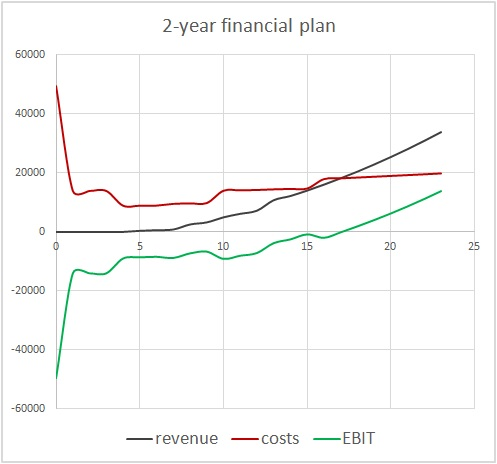
\includegraphics[width=0.7\textwidth]{financials}
\caption{Umsatz, Kosten und EBIT im neutralen Fall der Umsatzentwicklung}
\label{fig:financials1}
\end{figure}

\subsection{Detaillierte Finanzplanung}
Im Folgeden werden die Details des Finanzplans anhand des neutralen Szenarios näher betrachtet. Hier wird der Break-Event-Punkt in Monat 18 erreicht. In der Betrachtung der Kosten werden auch die Umsatzgebühren des Microtransaction-Dienstleisters PayPal berücksichtigt. In Abbildung \ref{fig:financials2} werden die einzelnen Kostenarten sowie Umsatzquellen und zusätzliche Parameter aufgeführt, die ein neutrales Umsatzszenario beschreiben. 
\begin{figure}[h!]
\centering
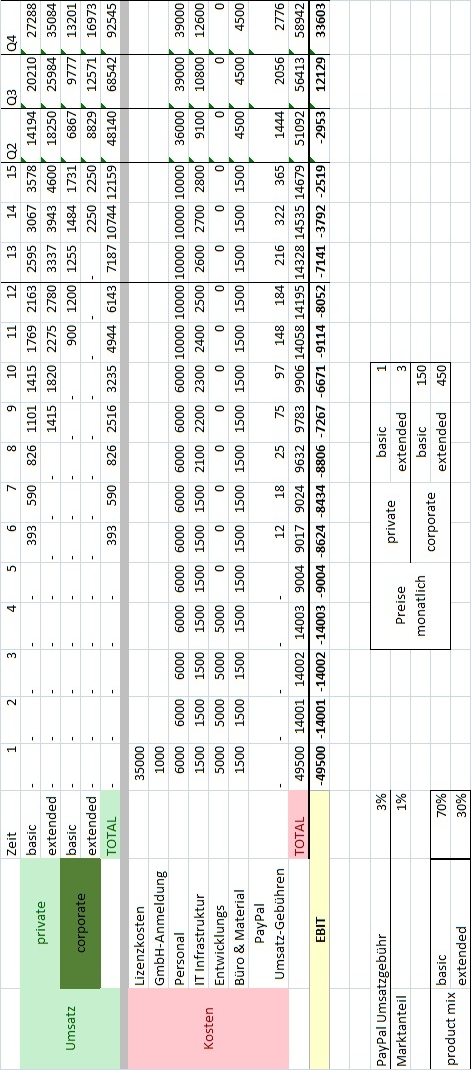
\includegraphics[width=0.6\textwidth]{finance-table}
\caption{Detaillierter Finanzplan für das neutrale Umsatz-Szenario.}
\label{fig:financials2}
\end{figure}
\\
\\
\\
\\
\\
\\
\\
\\
\\
\section{Schlusswort}
Das Gründerteam von SemLit ist zuversichtlich, dass Sie von unserem Erfolg überzeugt sind. Wir blicken entschlossen in die Zukunft und freuen uns auf eine erfolgreiche Zusammenarbeit. 
\\
\\
\\
\\
\\
\\
\\
\\
Igor Tseyzer und Artem Schumilin

\newpage




\end{document}